\section{Evaluation}
\label{evaluation}

We implemented\footnote{The project repository: \url{https://github.com/kajigor/uKanren_transformations/}. Access date: 28.02.2021} the conservative partial deduction for \mk and compared it with the \ecce partial deduction system.
\ecce is designed for \pro programming language and cannot be directly applied for programs, written in \mk.
Nevertheless, the languages show resemblance, and it is valuable to check if the existing methods for \pro can be used directly in the context of relational programming.
To be able to compare our approach with \ecce, we converted each input program first to the pure subset of \pro, then specialized it with \ecce, and then we converted the result back to \mk.
The conversion to \pro is a simple syntactic conversion. In the conversion from \pro to \mk, for each Horn clause a conjunction is generated in which unifications are placed before any relation call.
All programs are run as \mk programs in our experiments.

We chose two problems for our study: evaluation of a subset of propositional formulas and typechecking for a simple language.
The problems illustrate the approach of using relational interpreters to solve search problems~\cite{lozov2019relational}.
For both these problems we considered several possible implementations in \mk which highlight different aspects relevant in specialization.

The \lstinline{eval$^o$} relation implements an evaluator of a subset of propositional formulas described in the section~\ref{example}.
We consider four different implementations of this relation to explore how the way the program is implemented can affect the quality of specialization.
Depending on the implementation, \ecce generates programs of varying performance, while the execution times of the programs generated by our approach are similar.

The \lstinline{typecheck$^o$} relation implements a typechecker for a tiny expression language.
We consider two different implementations of this relation: one written by hand and the other generated from the functional program.
We demonstrate how much these implementations differ in terms of performance before and after specialization.

In this study we measured the execution time for the sample queries, averaging them over multiple runs.
We also measured the number of unifications done in search of each individual answer.
All examples of \mk relations in this paper are written in \oc.
The queries were run on a laptop running Ubuntu 18.04 with quad core Intel Core i5 2.30GHz CPU and 8 GB of RAM.

The tables and graphs use the following denotations.
\emph{Original} represents the execution time of a program before any transformations were applied; \emph{ECCE}~--- of the program specialized by \ecce with default conjunctive control setting; \emph{ConsPD}~--- of the program specialized by our approach.

\subsection{Evaluator of Logic Formulas}

The relation \lstinline{eval$^o$} describes an evaluation of a propositional formula under given variable assignments presented in section~\ref{example}.
We specialize the \lstinline{eval$^o$} relation to synthesize formulas which evaluate to \lstinline{true}.
To do so, we run the specializer for the goal with the last argument fixed to \lstinline{true}, while the first two arguments remain free variables.
Depending on the way the \lstinline{eval$^o$} is implemented, different specializers generate significantly different residual programs.

\subsubsection{The Order of Relation Calls}

One possible implementation of the \lstinline{eval$^o$} relation is presented in Listing~\ref{eval:last}.
Here the relation \lstinline{elem$^o$ s v res} unifies \lstinline{res} with the value of the variable \lstinline{v} in the list \lstinline{s}.
The relations \lstinline{and$^o$}, \lstinline{or$^o$}, and \lstinline{not$^o$} encode corresponding boolean connectives.

\begin{figure*}[!t]
  \centering
  \begin{minipage}{0.95\textwidth}
    \begin{lstlisting}[label={eval:last}, caption={Evaluator of formulas with boolean operation last}, captionpos=b, frame=tb]
  let rec eval$^o$ s fm res = conde [fresh (x y z v w) (
      (fm === conj x y /\ eval$^o$ s x v /\  eval$^o$ s y w /\  and$^o$ v w res);
      (fm === disj x y /\ eval$^o$ s x v /\  eval$^o$ s y w /\  or$^o$   v w res);
      (fm === neg x    /\ eval$^o$ s x v /\  not$^o$ v res));
      (fm === var v    /\ elem$^o$ s v res)]
    \end{lstlisting}
  \end{minipage}
  \begin{minipage}{0.95\textwidth}
    \begin{lstlisting}[label={eval:fst}, caption={Evaluator of formulas with boolean operation second}, captionpos=b, frame=tb]
  let rec eval$^o$ s fm res = conde [fresh (x y z v w) (
      (fm === conj x y /\ and$^o$ v w res /\  eval$^o$ s x v /\  eval$^o$ s y w);
      (fm === disj x y /\ or$^o$   v w res /\ eval$^o$ s x v /\  eval$^o$ s y w);
      (fm === neg x    /\ not$^o$ v res   /\ eval$^o$ s x v);
      (fm === var v    /\ elem$^o$ s v res))]
    \end{lstlisting}
  \end{minipage}
\end{figure*}

Note, the calls to boolean relations \lstinline{and$^o$}, \lstinline{or$^o$}, and \lstinline{not$^o$} are placed last within each conjunction.
This poses a challenge for the CPD-based specializers such as \ecce.
Conjunctive partial deduction unfolds relation calls from left to right, so when specializing this relation for running backwards (i.e. considering the goal \lstinline{eval$^o$ s fm true}), it fails to propagate the direction data onto recursive calls of \lstinline{eval$^o$}.
Knowing that \lstinline{res} is \lstinline{true}, we can conclude that in the call \lstinline{and$^o$ v w res} variables \lstinline{v} and \lstinline{w} have to be \lstinline{true} as well.
There are three possible options for these variables in the call \lstinline{or$^o$ v w res} and one for the call \lstinline{not$^o$}.
These variables are used in recursive calls of \lstinline{eval$^o$} and thus restrict the result of driving.
CPD fails to recognize this, and thus unfolds recursive calls of \lstinline{eval$^o$} applied to fresh variables.
It leads to over-unfolding, large residual programs and poor performance.

The conservative partial deduction first unfolds those calls which are selected according to the heuristic.
Since exploring the implementations of boolean connectives makes more sense, they are unfolded before recursive calls of \lstinline{eval$^o$}.
The way conservative partial deduction treats this program is the same as it treats the other implementation in which boolean connectives
are moved to the left, as shown in Listing~\ref{eval:fst}.
This program is easier for \ecce to specialize which demonstrates how unequal the behaviour of CPD for similar programs is.

\subsubsection{Unfolding of Complex Relations}

Depending on the way a relation is implemented, it may take a different number of driving steps to reach the point when any useful information is derived through its unfolding.
Partial deduction tries to unfold every relation call unless it is unsafe, but not all relation calls serve to restrict the search space and thus should be unfolded.
In the implementation of \lstinline{eval$^o$} boolean connectives can effectively restrict variables within the conjunctions and should be unfolded until they do.
But depending on the way they are implemented, the different number of driving steps should be performed for that.
The simplest way to implement these relations is by mimicking a truth table as demonstrated by the implementation of \lstinline{not$^o$} in Listing~\ref{not:table}.
It is enough to unfold such relation calls once to derive useful information about variables.

\begin{figure*}[!t]
  \centering
  \begin{minipage}{0.5\textwidth}
    \begin{lstlisting}[label={not:table}, caption={Implementation of boolean not$^o$ as a table}, captionpos=b, frame=tb]
      let not$^o$ x y = conde [
         (x === true /\ y === false;
          x === false /\ y === true)]
    \end{lstlisting}
  \end{minipage}
  \begin{minipage}{0.8\textwidth}
    \begin{lstlisting}[label={not:nando}, caption={Implementation of boolean operations via nand$^o$}, captionpos=b, frame=tb]
  let not$^o$   x y = nand$^o$ x x y
  let or$^o$   x y z = nand$^o$ x x xx /\  nand$^o$ y y yy /\ nand$^o$ xx yy z
  let and$^o$ x y z = nand$^o$ x y xy /\   nand$^o$ xy xy z
  let nand$^o$ a b c = conde [
    ( a === false /\ b === false /\ c === true );
    ( a === false /\ b === true  /\ c === true );
    ( a === true  /\ b === false /\ c === true );
    ( a === true  /\ b === true  /\ c === false)]
    \end{lstlisting}
  \end{minipage}
\end{figure*}

The other way to implement boolean connectives is to express them using a single basic boolean relation such as \lstinline{nand$^o$} which is, in turn, has a table-based
implementation (see Listing~\ref{not:nando}). It will take several sequential unfoldings to derive that variables \lstinline{v} and \lstinline{w} should
be \lstinline{true} when considering a call \lstinline{and$^o$ v w true} implemented via a basic relation.
Conservative partial deduction drives the selected call until it derives useful substitutions for the variables involved while CPD with deterministic unfolding may fail to do so.


\subsubsection{Evaluation Results}

In our study we considered 4 implementations of \lstinline{eval$^o$} summed up in the Table~\ref{tbl:eval}. They differ in the way the boolean connectives are implemented (see column \emph{Implementation}) and whether they are placed before or after the recursive calls to \lstinline{eval$^o$} (see column \emph{Placement}).
These four implementations are very different from the  standpoint of \ecce.

\begin{table}[!h]
    \centering
    \begin{tabular}{c||c||c}
                      & Implementation & Placement \\ \hline\hline
    \emph{FirstPlain} & table-based    & before \\ \hline
    \emph{LastPlain}  & table-based    & after  \\ \hline
    \emph{FirstNando} & via nand$^o$   & before \\ \hline
    \emph{LastNando}  & via nand$^o$   & after  \\
    \end{tabular}

  \caption{Different implementations of eval$^o$}
  \label{tbl:eval}
\end{table}

We measured the time necessary to generate $1000$ formulas over two variables which evaluate to \lstinline{true} (averaged over 10 runs).
The results are presented in Fig.~\ref{fig:eval}.

\begin{figure}[!t]
  \centering
  \begin{subfigure}[c]{0.35\textwidth}
    \centering
    \begin{tabular}{e{1cm}||c|c|c}
               & Original & \ecce & ConsPD \\ \hline\hline
      \emph{FirstPlain} & 1.59s & 1.61s & 0.92s \\ \hline
      \emph{FirstNando} & 1.43s & 2.24s & 0.96s \\ \hline
      \emph{LastPlain}  & 0.98s & 1.43s & 0.97s \\ \hline
      \emph{LastNando}  & 1.09s & 1.54s & 0.91s
    \end{tabular}
  \end{subfigure}
  \hfill
  \begin{subfigure}[c]{0.58\textwidth}
    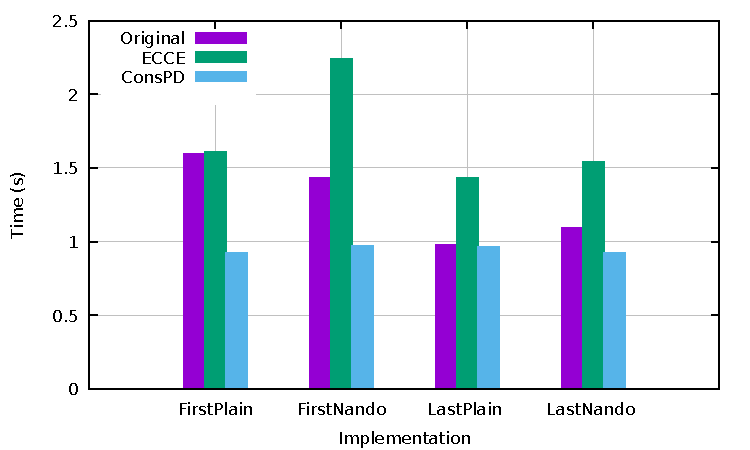
\includegraphics[width=\textwidth]{data/propEval/prop.pdf}
  \end{subfigure}
  \caption{Execution time of eval$^o$}
  \label{fig:eval}
\end{figure}

Conservative partial deduction generates  programs with comparable performance for all four implementations, while the quality of \ecce specialization differs significantly.
\ecce worsens performance for every implementation as compared to the original program.
ConsPD do not worsen performance for any implementation.
Its effect is most significant for the implementations in which the boolean connectives are placed first within conjunctions.

\subsubsection{The Order of Answers}

It is important to note that different implementations of the same \mk relation produce answers in different orders.
Nevertheless, since \mk search is complete, all answers will be found eventually.
Unfortunately, it is not guaranteed that the first 1000 formulas generated with different implementations of \lstinline{eval$^o$} will be the same.
For example, $983$ formulas are the same among the first $1000$ formulas generated by the Original \emph{FirstPlain} relation and the same relation after the ConsPD transformation.
At the same time, only $405$ formulas are the same between the Original and \ecce \emph{LastNando} relations.

The reason why implementations differ so much in the order of the answers stems from the canonical search strategy employed in \mk.
Most \mk implementations employ \emph{interleaving} search~\cite{10.1145/1090189.1086390} which is left-biased.
It means that the leftmost disjunct in a relation is being executed longer than the disjunct on the right.
This property is not local which makes it very hard to estimate the performance of a given relation.

In practice it means that if a specializer reorders disjuncts, then the performance of relations after specialization may be unpredictable.
For example, by putting the disjuncts of the \lstinline{eval$^o$} relation in the opposite order, one produces a relation which runs much faster than the original, but it generates completely different formulas at the same time.
Most of the first 1000 formulas in this case are multiple negations of a variable, while the original relation produces more diverse set of answers.
Computing a negation of a formula only takes one recursive \lstinline{eval$^o$} call thus finding such answers is faster than conjunctions and disjunctions.
Meanwhile, the formulas generated by the reordered relation are less diverse and may be of less interest.

Although neither \ecce nor ConsPD reorder disjuncts, they remove disjuncts which cannot succeed.
Thus they influence the order of answers and performance of relations.
Both methods reduce the number of unifications needed to compute each individual answer thus performing specialization.
In general, it is not possible to guarantee the same order of answers after specialization.
Exploring how different specializations influence the execution order is a fascinating direction for future research.


\subsection{Typechecker-Term Generator}

This relation implements a typechecker for a tiny expression language.
Being executed in the backward direction it serves as a generator of terms of the given type.
The abstract syntax of the language is presented below.
The variables are represented with de Bruijn indices, thus let-binding does not specify which variable is being bound.

\[\begin{array}{lllll}
  type \ term = &\ BConst \ of \ Bool &| \ IConst \ of \ Int &| \ Var \ of \ Int & \\
  & | \ term + term &| \ term * term &| \ term = term &| \ term < term \\
  &| \ \underline{let} \ term \ \underline{in} \ term
  &\multicolumn{2}{l}{| \ \underline{if} \ term \ \underline{then} \ term \ \underline{else} \ term} &
\end{array}\]

The typing rules are straightforward and are presented in Fig.~\ref{fig:typing}.
Boolean and integer constants have the corresponding types regardless of the environment.
Only terms of type integer can be summed up, multiplied or compared by less-than operator.
Any terms of the same type can be checked for equality.
Addition and multiplication of two terms of suitable types have integer type, while comparisons have boolean type.
If-then-else expression typechecks only if its condition is of type boolean, while both then- and else-branches have the same type.
An environment $\Gamma$ is an ordered list, in which the $i$-th element is the type of the variable with the $i$-th de Bruijn index.
To typecheck a let-binding, first, the term being bound is typechecked and is added in the beginning of the environment $\Gamma$, and then the body is typechecked in the context of the new environment.
Typechecking a variable with the index $i$ boils down to getting an $i$-th element of the list.

\begin{figure}[!h]
  \setlength{\tabcolsep}{0.4cm}
  \centering
  \begin{tabular}{c c c}
    \infer[]{\Gamma \vdash IConst \ i : Int}{} &
    \infer[]{\Gamma \vdash BConst \ b : Bool}{}  &
    \infer[\Gamma \lbrack v \rbrack \equiv \tau]{\Gamma \vdash Var \ v : \tau}{} \vspace{0.5cm}
    \\
    \infer[]{\Gamma \vdash t + s : Int}{\Gamma \vdash t : Int, \Gamma \vdash  s : Int}  \vspace{0.5cm} &
    \infer[]{\Gamma \vdash t = s : Bool}{\Gamma \vdash t : \tau, \Gamma \vdash  s : \tau} &
    \infer[]{\Gamma \vdash \underline{let} \ v \ b : \tau}{\Gamma \vdash v : \tau_v, \ (\tau_v :: \Gamma) \vdash b : \tau}
      \\

      \infer[]{\Gamma \vdash t * s : Int}{\Gamma \vdash t : Int, \Gamma \vdash  s : Int}  &
    \infer[]{\Gamma \vdash t < s : Bool}{\Gamma \vdash t : Int, \Gamma \vdash  s : Int} \vspace{0.5cm} &
      \infer[]{\Gamma \vdash \underline{if} \ c \ \underline{then} \ t \ \underline{else} \ s : \tau}{\Gamma \vdash c : Bool, \Gamma \vdash t : \tau, \Gamma \vdash s : \tau}
  \end{tabular}
  \vspace{-0.3cm}
  \caption{Typing rules implemented in typecheck$^o$ relation}
  \label{fig:typing}
\end{figure}


We compared two implementations of these typing rules.
The first one is obtained by unnesting of a functional program as described in~\cite{lozov2019relational} (\emph{Generated}).
It is worth noting that the unnesting introduces a lot of redundancy in the form of extra unifications and thus creates programs which are very inefficient.
Thus we contrast this implementation with the program hand-written in \oc (\emph{Hand-written}).
Each implementation has been specialized with ConsPD and \ecce.
We measured the time needed to generate 1000 closed terms of type integer (see Fig.~\ref{tbl:type}).


\begin{figure}[!h]
  \begin{subfigure}[c]{0.55\textwidth}
    \centering
    \begin{tabular}{c||c|c|c}
                          & Original & \ecce & ConsPD  \\ \hline\hline
      \emph{Hand-written} & 0.92s    & 0.22s & 0.34s   \\ \hline
      \emph{Generated}    & 11.46s   & 0.38s & 0.29s
      \end{tabular}
  \end{subfigure}
  \hfill
  \begin{subfigure}[c]{0.45\textwidth}
    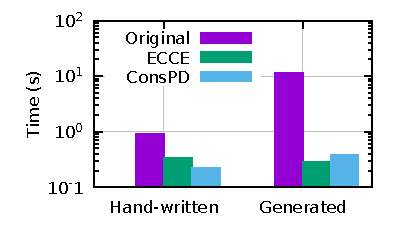
\includegraphics[width=\textwidth]{data/lTypecheck/ltypelog.pdf}
  \end{subfigure}
  \caption{Execution  time of generating 1000 closed terms of type integer}
  \label{tbl:type}
\end{figure}

As expected, the generated program is far slower than the hand-written.
The principal difference between these two implementations is that the generated program contains a certain redundancy introduced by unnesting.
For example, typechecking of the sum of two terms in the hand-written implementation consists of a single conjunction (see Listing~\ref{type:hand}) while the generated program is far more complicated and also uses a special relation \lstinline{typeEq$^o$} to compare types (see Listing~\ref{type:gen}).

\begin{figure*}[!h]
  \centering
    \begin{lstlisting}[label={type:hand}, caption={A fragment of hand-written typechecker}, captionpos=b, frame=tb]
  let rec typecheck$^o$ gamma term res = conde [
    ...
    fresh (x y) ((term === x + y /\
       typecheck$^o$ gamma x (some integer) /\
       typecheck$^o$ gamma y (some integer) /\
       res === (some integer)));
    ...]
    \end{lstlisting}
\end{figure*}


\begin{figure*}[!t]
  \centering
    \begin{lstlisting}[label={type:gen}, caption={A fragment of generated typechecker}, captionpos=b, frame=tb]
let rec typecheck$^o$ gamma term res = conde [
  ...
  fresh (x y t1 t2) ((term === x + y /\
    conde [
      typecheck$^o$ gamma x none       /\ res === none;
      typecheck$^o$ gamma x (some t1) /\
        typecheck$^o$ gamma y none     /\ res === none;
      typecheck$^o$ gamma x (some t1) /\  typecheck$^o$ gamma y (some t2) /\
        typeEq$^o$ t1 integer true     /\ typeEq$^o$ t2 integer true /\
        res === (some integer);
    ])
  ...]
    \end{lstlisting}
\end{figure*}

Most of the redundancy of the generated program is removed by specialization with respect to the known type of the term.
This is why both implementations have comparable speed after specialization.
\ecce shows bigger speedup for the hand-written program than ConsPD and vice versa for the generated implementation.
We believe that this difference can be explained by too much unfolding.
\ecce performs a lot of excessive unfolding for the generated program and only barely changes the hand-written program.
At the same time ConsPD specializes both implementations to comparable programs performing average amount of unfolding.
This shows that the heuristic we presented gives more stable, although not the best, results.


\subsection{Tupling and Deforestation}


\begin{figure*}[!t]
  \centering
  \begin{minipage}{0.7\textwidth}
    \begin{lstlisting}[label={doubleApp}, caption={Inefficient implementation of concatenation of three lists}, captionpos=b, frame=tb]
    let doubleAppend$^o$ x y z res = fresh (t) (
        append$^o$ x y t /\ append$^o$ t z res )

    let append$^o$ x y res = conde [ fresh (h t r) (
        ( x === [] /\ res === y );
        ( x === h % t /\ append$^o$ t y r /\ res === h % r ))]
    \end{lstlisting}
  \end{minipage}
\end{figure*}

\begin{figure*}[!t]
  \centering
  \begin{minipage}{0.7\textwidth}
    \begin{lstlisting}[label={maxlen}, caption={Inefficient implementation of maxLength$^o$}, captionpos=b, frame=tb]
    let maxLength$^o$ x m l = fresh (t) (
        max$^o$ x m /\ length$^o$ x l )

    let length$^o$ x l = conde [ fresh (h t r) (
        ( x === [] /\ l === zero );
        ( x === h % t /\ length$^o$ t r /\ l === succ r ))]

    let max$^o$ x m = max$_1^o$ x zero m
    let rec max$_1^o$ x n m = fresh (h t) ( conde [
        (x === [] /\ m === n);
        (x === h % t) /\ (conde [
          (le$^o$ h n true /\  max$_1^o$ t n m);
          (gt$^o$ h n true /\  max$_1^o$ t h m)])])
    \end{lstlisting}
  \end{minipage}
\end{figure*}

Tupling and deforestation are among the important transformations conjunctive partial deduction is capable of.
Deforestation is often demonstrated by the \lstinline{doubleAppend} program which concatenates three lists by calling the concatenation relation \lstinline{append} twice in a conjunction (see Listing~\ref{doubleApp}).
The two calls to \lstinline{append} lead to double traversal of the first list, which is inefficient.
The program may be transformed in such a way so as to only traverse the first list once (see~\cite{de1999conjunctive} for details), which conjunctive partial deduction does.

Conjunctive partial deduction achieves this effect by considering the conjunction of two \lstinline{append} calls as a whole.
It first unfolds the leftmost call, propagates the computed substitutions onto the rightmost call, and then unfolds the rightmost call in the context of the substitutions.
When the first list is not empty, then this leads to discovering a renaming of a conjunction of two \lstinline{append} calls.
By renaming this conjunction into a new predicate, deforestation is achieved in this example.

Unfortunately, conservative partial deduction does not succeed at this transformation on this example.
This happens because ConsPD splits the conjunction of two calls to \lstinline{append}, since none of them is selected by the less branching heuristic.
Splitting the conjunction leads to information loss and makes it so there is no renaming of the whole conjunction in the process tree.

The similar thing happens when considering the common example on which tupling is demonstrated in literature on CPD: the \lstinline{maxLength} program.
The original implementation of this program computes the maximum element of the list along with the length of the list by conjunction of two calls to the corresponding relations \lstinline{max} and \lstinline{length} (see Listing.~\ref{maxlen}).
This implementation also traverses the input list twice when run in the forward direction.
By tupling, this program may be transformed so that the list is traversed once and both the maximum value and the length of the list are computed simultaneously, and CPD is capable to achieve this transformation with the default settings.
Conservative partial deduction also splits too much too early and thus fails to yield any useful transformation for this program.

It is worth noting that the fact that determinate unfolding performed by CPD plays a huge role in these examples.
The default unfolding strategy implemented in \ecce allows for only a single non-determinate unfolding per a local control tree.
When considering conjunctions \lstinline{append$^o$ x y t /\ append$^o$ t z res} and \lstinline{max$^o$ x m /\ length$^o$ x l}, CPD unfolds the leftmost call which produces several branches in the tree.
The rightmost call is only considered, if unfolding of its conjunction with the result of unfolding of the leftmost call produces only one result.
This indeed happens in these two examples.
If it was not to happen, then the conjunction would have been split at the global level and no deforestation or tupling would have been achieved.
It is not that hard to modify the examples in such a way so that CPD fails to transform them in a meaningful way.
For example, one extra disjunct can be added into the \lstinline{append$^o$} relation, or the calls to \lstinline{max$^o$} and \lstinline{length$^o$} may be reordered.
This is an evidence of how non-trivial and fragile these transformers are.
More research should be done to make sure useful transformations are possible for more input programs.


